\documentclass[tikz,border=10pt]{standalone}
\usepackage{tikz}
\usetikzlibrary{shapes,arrows,positioning,calc,decorations.pathmorphing,backgrounds,shadows,fit,matrix}

% Define colors
\definecolor{primaryblue}{RGB}{0,102,204}
\definecolor{secondarygreen}{RGB}{46,204,113}
\definecolor{accentorange}{RGB}{255,127,0}
\definecolor{warningred}{RGB}{231,76,60}
\definecolor{lightgray}{RGB}{236,240,241}
\definecolor{darkgray}{RGB}{52,73,94}

\begin{document}
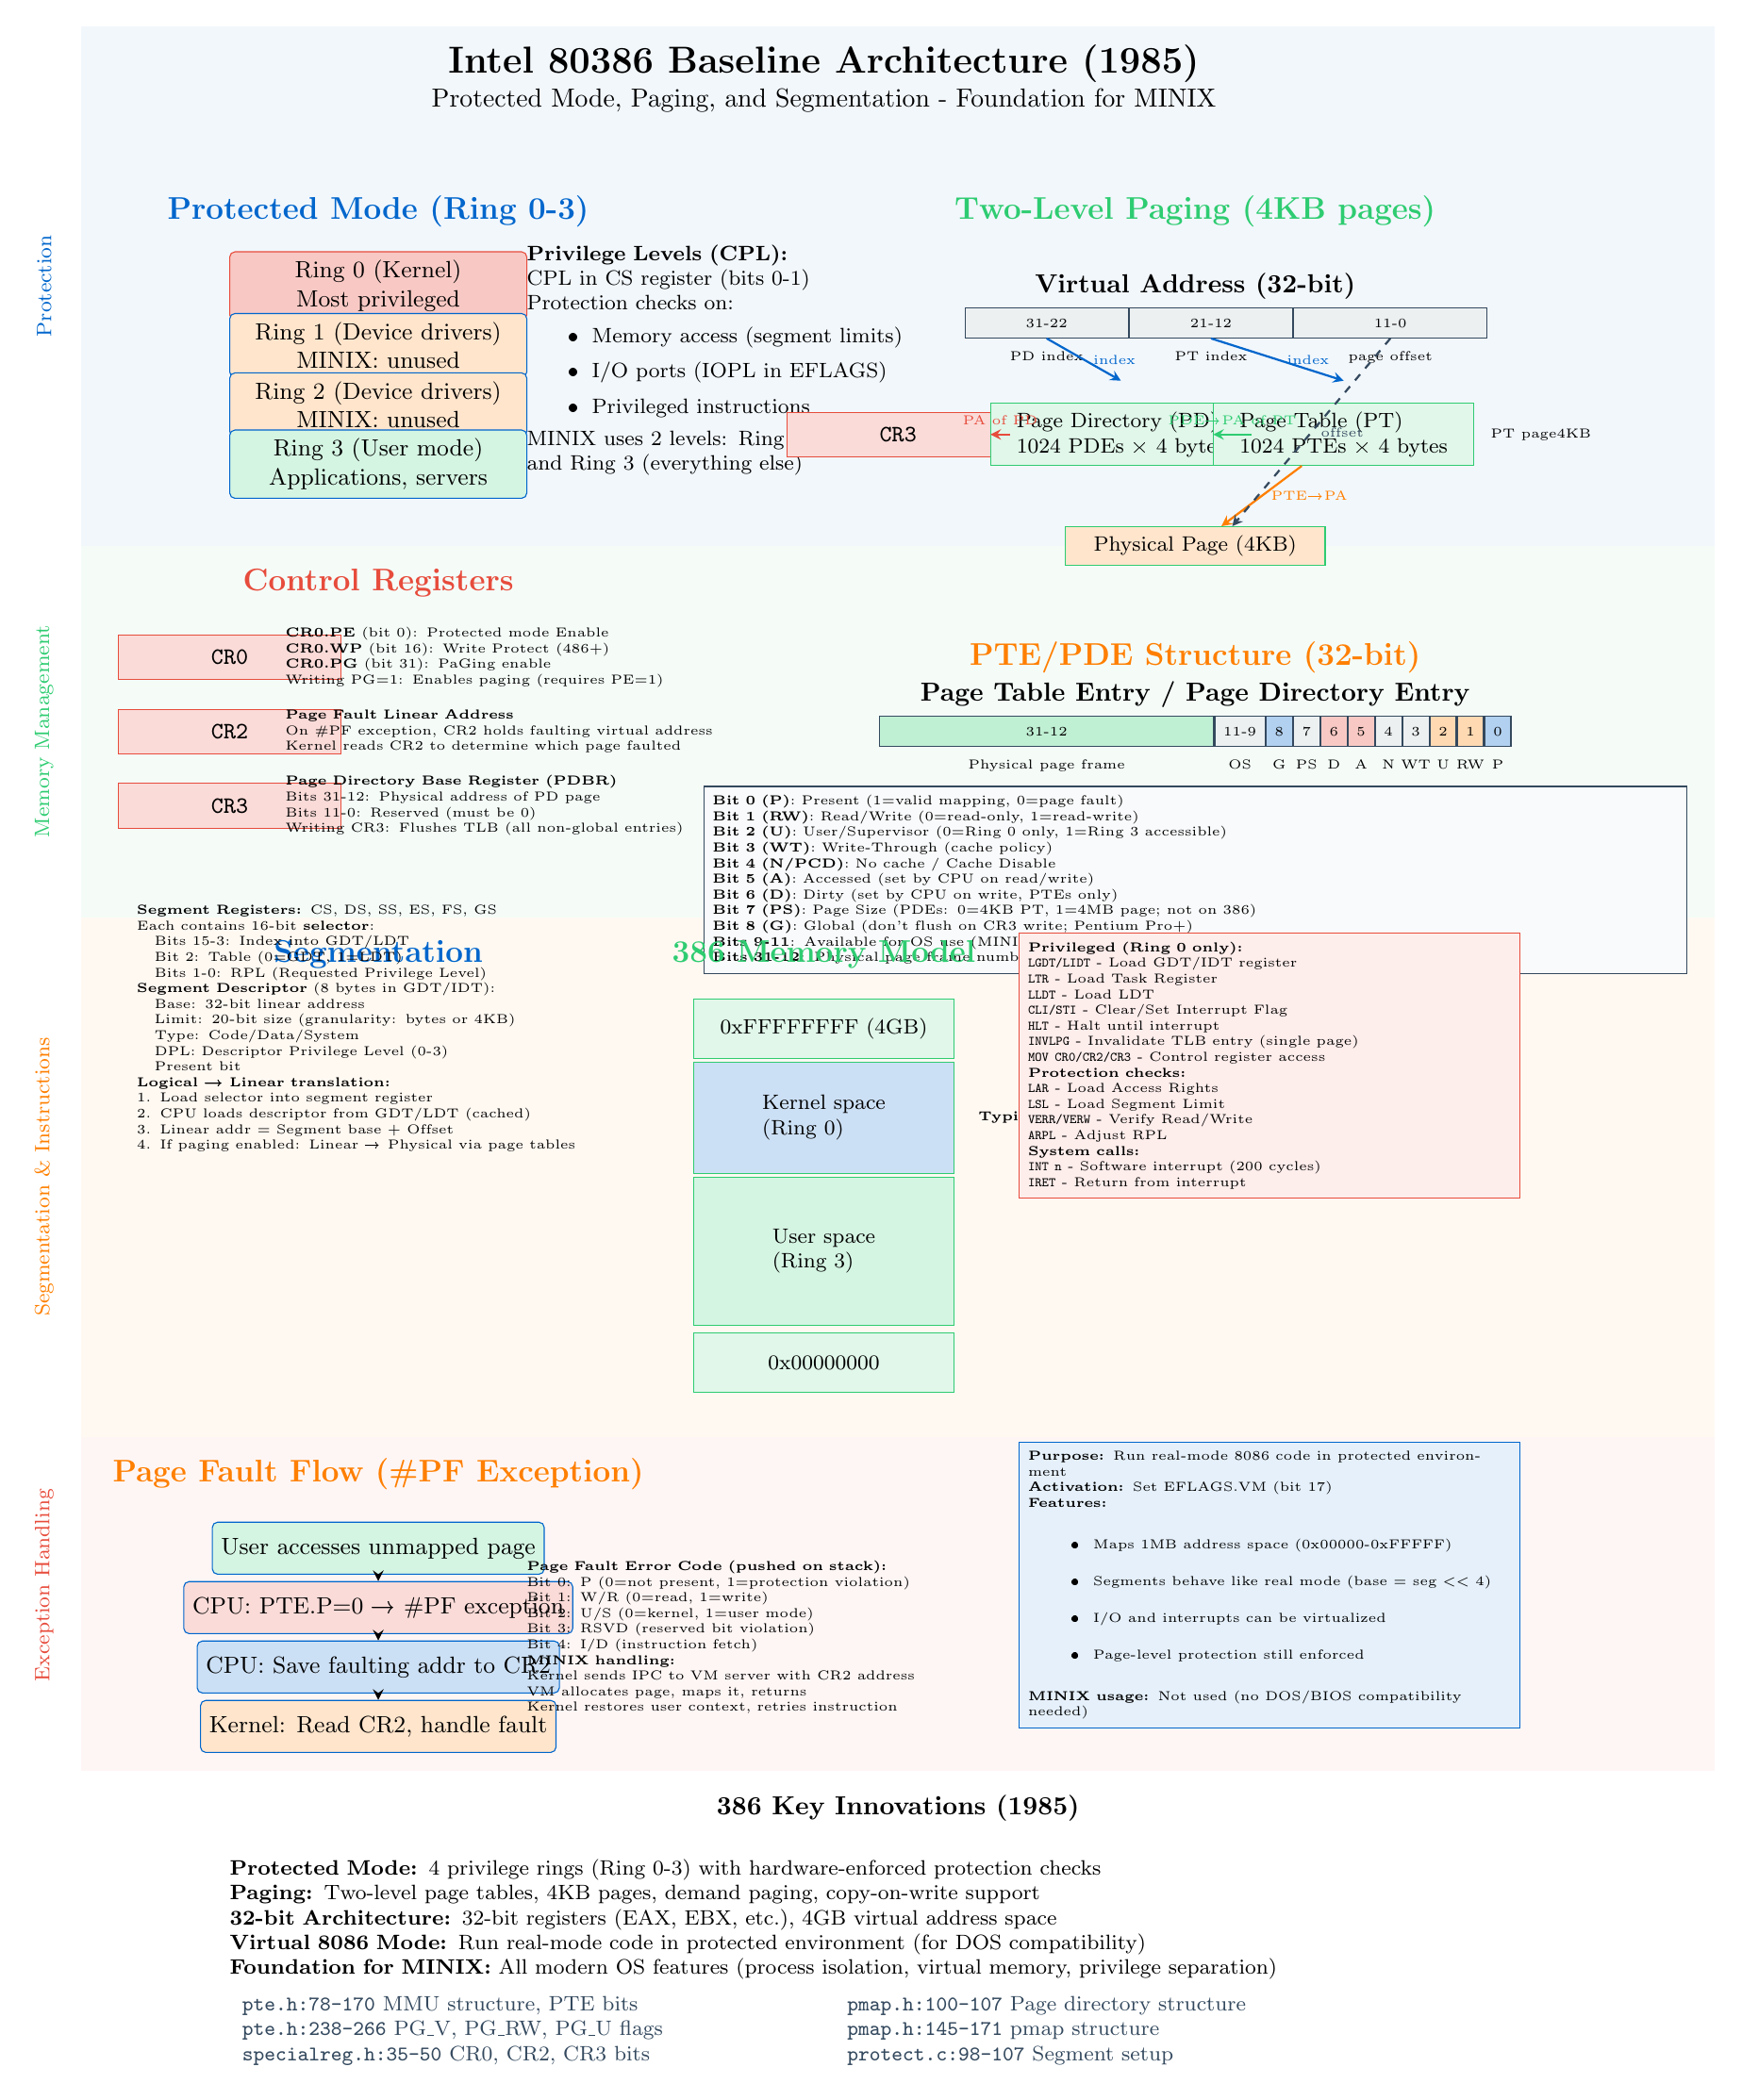
\begin{tikzpicture}[
    box/.style={rectangle, rounded corners=2pt, draw=primaryblue, fill=primaryblue!15, minimum width=4cm, minimum height=0.7cm, font=\small, align=center},
    regbox/.style={rectangle, draw=warningred, fill=warningred!20, minimum width=3cm, minimum height=0.6cm, font=\small\ttfamily, align=center},
    membox/.style={rectangle, draw=secondarygreen, fill=secondarygreen!15, minimum width=3.5cm, minimum height=0.5cm, font=\footnotesize, align=left},
    bitbox/.style={rectangle, draw=darkgray, fill=lightgray, minimum width=0.4cm, minimum height=0.4cm, font=\tiny},
    arrow/.style={->, >=stealth, thick},
    label/.style={font=\footnotesize}
]

% Title
\node[font=\Large\bfseries] at (10, 22) {Intel 80386 Baseline Architecture (1985)};
\node[font=\normalsize] at (10, 21.5) {Protected Mode, Paging, and Segmentation - Foundation for MINIX};

%% PROTECTED MODE - Ring levels
\node[font=\bfseries\large, primaryblue] at (4, 20) {Protected Mode (Ring 0-3)};

\node[box, fill=warningred!30, draw=warningred] (ring0) at (4, 19) {Ring 0 (Kernel)\\Most privileged};
\node[box, fill=accentorange!20] (ring1) at (4, 18.2) {Ring 1 (Device drivers)\\MINIX: unused};
\node[box, fill=accentorange!20] (ring2) at (4, 17.4) {Ring 2 (Device drivers)\\MINIX: unused};
\node[box, fill=secondarygreen!20] (ring3) at (4, 16.6) {Ring 3 (User mode)\\Applications, servers};

\node[label, text width=6cm, align=left] at (9, 18) {
\textbf{Privilege Levels (CPL):}\\
CPL in CS register (bits 0-1)\\
Protection checks on:
\begin{itemize}
\item Memory access (segment limits)
\item I/O ports (IOPL in EFLAGS)
\item Privileged instructions
\end{itemize}
MINIX uses 2 levels: Ring 0 (kernel) \\and Ring 3 (everything else)
};

%% CONTROL REGISTERS
\node[font=\bfseries\large, warningred] at (4, 15) {Control Registers};

% CR0
\node[regbox] (cr0) at (2, 14) {CR0};
\node[label, text width=6.5cm, align=left, font=\tiny] at (6, 14) {
\textbf{CR0.PE} (bit 0): Protected mode Enable\\
\textbf{CR0.WP} (bit 16): Write Protect (486+)\\
\textbf{CR0.PG} (bit 31): PaGing enable\\
Writing PG=1: Enables paging (requires PE=1)
};

% CR2
\node[regbox] (cr2) at (2, 13) {CR2};
\node[label, text width=6.5cm, align=left, font=\tiny] at (6, 13) {
\textbf{Page Fault Linear Address}\\
On \#PF exception, CR2 holds faulting virtual address\\
Kernel reads CR2 to determine which page faulted
};

% CR3
\node[regbox] (cr3) at (2, 12) {CR3};
\node[label, text width=6.5cm, align=left, font=\tiny] at (6, 12) {
\textbf{Page Directory Base Register (PDBR)}\\
Bits 31-12: Physical address of PD page\\
Bits 11-0: Reserved (must be 0)\\
Writing CR3: Flushes TLB (all non-global entries)
};

%% TWO-LEVEL PAGING
\node[font=\bfseries\large, secondarygreen] at (15, 20) {Two-Level Paging (4KB pages)};

% Virtual address breakdown
\node[label, font=\bfseries] at (15, 19) {Virtual Address (32-bit)};

\node[bitbox, minimum width=2.2cm] (va_pd) at (13, 18.5) {31-22};
\node[label, font=\tiny, below=0.05cm of va_pd] {PD index};

\node[bitbox, minimum width=2.2cm, right=0cm of va_pd] (va_pt) {21-12};
\node[label, font=\tiny, below=0.05cm of va_pt] {PT index};

\node[bitbox, minimum width=2.6cm, right=0cm of va_pt] (va_offset) {11-0};
\node[label, font=\tiny, below=0.05cm of va_offset] {page offset};

% Translation flow
\node[regbox] (cr3_flow) at (11, 17) {CR3};

\node[membox] (pd) at (14, 17) {Page Directory (PD)\\1024 PDEs × 4 bytes};
\node[label, font=\tiny, right=0.1cm of pd] {PD page\\4KB};

\node[membox] (pt) at (17, 17) {Page Table (PT)\\1024 PTEs × 4 bytes};
\node[label, font=\tiny, right=0.1cm of pt] {PT page\\4KB};

\node[membox, fill=accentorange!20] (phys) at (15, 15.5) {Physical Page (4KB)};

% Arrows showing translation
\draw[arrow, warningred] (cr3_flow) -- (pd) node[midway, above, font=\tiny] {PA of PD};
\draw[arrow, primaryblue] (va_pd.south) -- ($(pd.north) + (0, 0.3)$) node[midway, right, font=\tiny] {index};
\draw[arrow, secondarygreen] (pd) -- (pt) node[midway, above, font=\tiny] {PDE→PA of PT};
\draw[arrow, primaryblue] (va_pt.south) -- ($(pt.north) + (0, 0.3)$) node[midway, right, font=\tiny] {index};
\draw[arrow, accentorange] (pt) -- (phys) node[midway, right, font=\tiny] {PTE→PA};
\draw[arrow, darkgray, dashed] (va_offset.south) -- ($(phys.north) + (0.5, 0)$) node[midway, right, font=\tiny] {offset};

%% PTE/PDE BIT LAYOUT
\node[font=\bfseries\large, accentorange] at (15, 14) {PTE/PDE Structure (32-bit)};

% Bit layout
\node[label, font=\bfseries] at (15, 13.5) {Page Table Entry / Page Directory Entry};

% Physical frame
\node[bitbox, minimum width=4.5cm, fill=secondarygreen!30] (pte_frame) at (13, 13) {31-12};
\node[label, font=\tiny, below=0.05cm of pte_frame] {Physical page frame};

% OS available
\node[bitbox, minimum width=0.65cm, right=0cm of pte_frame] (pte_avail) {11-9};
\node[label, font=\tiny, below=0.05cm of pte_avail] {OS};

% G
\node[bitbox, minimum width=0.35cm, right=0cm of pte_avail, fill=primaryblue!30] (pte_g) {8};
\node[label, font=\tiny, below=0.05cm of pte_g] {G};

% PS/PAT
\node[bitbox, minimum width=0.35cm, right=0cm of pte_g] (pte_ps) {7};
\node[label, font=\tiny, below=0.05cm of pte_ps] {PS};

% D
\node[bitbox, minimum width=0.35cm, right=0cm of pte_ps, fill=warningred!30] (pte_d) {6};
\node[label, font=\tiny, below=0.05cm of pte_d] {D};

% A
\node[bitbox, minimum width=0.35cm, right=0cm of pte_d, fill=warningred!30] (pte_a) {5};
\node[label, font=\tiny, below=0.05cm of pte_a] {A};

% PCD
\node[bitbox, minimum width=0.35cm, right=0cm of pte_a] (pte_pcd) {4};
\node[label, font=\tiny, below=0.05cm of pte_pcd] {N};

% PWT
\node[bitbox, minimum width=0.35cm, right=0cm of pte_pcd] (pte_pwt) {3};
\node[label, font=\tiny, below=0.05cm of pte_pwt] {WT};

% U/S
\node[bitbox, minimum width=0.35cm, right=0cm of pte_pwt, fill=accentorange!30] (pte_u) {2};
\node[label, font=\tiny, below=0.05cm of pte_u] {U};

% R/W
\node[bitbox, minimum width=0.35cm, right=0cm of pte_u, fill=accentorange!30] (pte_rw) {1};
\node[label, font=\tiny, below=0.05cm of pte_rw] {RW};

% P
\node[bitbox, minimum width=0.35cm, right=0cm of pte_rw, fill=primaryblue!30] (pte_p) {0};
\node[label, font=\tiny, below=0.05cm of pte_p] {P};

% Bit descriptions
\node[rectangle, draw=darkgray, fill=lightgray!30, text width=13cm, align=left, font=\tiny] at (15, 11) {
\textbf{Bit 0 (P)}: Present (1=valid mapping, 0=page fault)\\
\textbf{Bit 1 (RW)}: Read/Write (0=read-only, 1=read-write)\\
\textbf{Bit 2 (U)}: User/Supervisor (0=Ring 0 only, 1=Ring 3 accessible)\\
\textbf{Bit 3 (WT)}: Write-Through (cache policy)\\
\textbf{Bit 4 (N/PCD)}: No cache / Cache Disable\\
\textbf{Bit 5 (A)}: Accessed (set by CPU on read/write)\\
\textbf{Bit 6 (D)}: Dirty (set by CPU on write, PTEs only)\\
\textbf{Bit 7 (PS)}: Page Size (PDEs: 0=4KB PT, 1=4MB page; not on 386)\\
\textbf{Bit 8 (G)}: Global (don't flush on CR3 write; Pentium Pro+)\\
\textbf{Bits 9-11}: Available for OS use (MINIX: tracking flags)\\
\textbf{Bits 31-12}: Physical page frame number (aligned to 4KB)
};

%% SEGMENTATION
\node[font=\bfseries\large, primaryblue] at (4, 10) {Segmentation};

\node[label, text width=6.5cm, align=left, font=\tiny] at (4, 9) {
\textbf{Segment Registers:} CS, DS, SS, ES, FS, GS\\
Each contains 16-bit \textbf{selector}:\\
\quad Bits 15-3: Index into GDT/LDT\\
\quad Bit 2: Table (0=GDT, 1=LDT)\\
\quad Bits 1-0: RPL (Requested Privilege Level)\\

\textbf{Segment Descriptor} (8 bytes in GDT/IDT):\\
\quad Base: 32-bit linear address\\
\quad Limit: 20-bit size (granularity: bytes or 4KB)\\
\quad Type: Code/Data/System\\
\quad DPL: Descriptor Privilege Level (0-3)\\
\quad Present bit\\

\textbf{Logical → Linear translation:}\\
1. Load selector into segment register\\
2. CPU loads descriptor from GDT/LDT (cached)\\
3. Linear addr = Segment base + Offset\\
4. If paging enabled: Linear → Physical via page tables
};

%% MEMORY MAP
\node[font=\bfseries\large, secondarygreen] at (10, 10) {386 Memory Model};

\node[membox, minimum height=0.8cm] (mem_4gb) at (10, 9) {0xFFFFFFFF (4GB)};
\node[membox, minimum height=1.5cm, fill=primaryblue!20] (mem_kernel) at (10, 7.8) {Kernel space\\(Ring 0)};
\node[membox, minimum height=2cm, fill=secondarygreen!20] (mem_user) at (10, 6) {User space\\(Ring 3)};
\node[membox, minimum height=0.8cm] (mem_0) at (10, 4.5) {0x00000000};

\node[label, font=\tiny, right=0.2cm of mem_kernel] {
\textbf{Typical split:}\\
3GB user / 1GB kernel\\
(MINIX uses flat model)
};

%% INSTRUCTIONS
\node[font=\bfseries\large, warningred] at (16, 10) {Key 386 Instructions};

\node[rectangle, draw=warningred, fill=warningred!10, text width=6.5cm, align=left, font=\tiny] at (16, 8.5) {
\textbf{Privileged (Ring 0 only):}\\
\texttt{LGDT/LIDT} - Load GDT/IDT register\\
\texttt{LTR} - Load Task Register\\
\texttt{LLDT} - Load LDT\\
\texttt{CLI/STI} - Clear/Set Interrupt Flag\\
\texttt{HLT} - Halt until interrupt\\
\texttt{INVLPG} - Invalidate TLB entry (single page)\\
\texttt{MOV CR0/CR2/CR3} - Control register access\\

\textbf{Protection checks:}\\
\texttt{LAR} - Load Access Rights\\
\texttt{LSL} - Load Segment Limit\\
\texttt{VERR/VERW} - Verify Read/Write\\
\texttt{ARPL} - Adjust RPL\\

\textbf{System calls:}\\
\texttt{INT n} - Software interrupt (200 cycles)\\
\texttt{IRET} - Return from interrupt
};

%% PAGE FAULT HANDLING
\node[font=\bfseries\large, accentorange] at (4, 3) {Page Fault Flow (\#PF Exception)};

\node[box, fill=secondarygreen!20] (pf1) at (4, 2) {User accesses unmapped page};
\node[box, fill=warningred!20] (pf2) at (4, 1.2) {CPU: PTE.P=0 → \#PF exception};
\node[box, fill=primaryblue!20] (pf3) at (4, 0.4) {CPU: Save faulting addr to CR2};
\node[box, fill=accentorange!20] (pf4) at (4, -0.4) {Kernel: Read CR2, handle fault};

\draw[arrow] (pf1) -- (pf2);
\draw[arrow] (pf2) -- (pf3);
\draw[arrow] (pf3) -- (pf4);

\node[label, text width=6cm, align=left, font=\tiny] at (9, 0.8) {
\textbf{Page Fault Error Code (pushed on stack):}\\
Bit 0: P (0=not present, 1=protection violation)\\
Bit 1: W/R (0=read, 1=write)\\
Bit 2: U/S (0=kernel, 1=user mode)\\
Bit 3: RSVD (reserved bit violation)\\
Bit 4: I/D (instruction fetch)\\

\textbf{MINIX handling:}\\
Kernel sends IPC to VM server with CR2 address\\
VM allocates page, maps it, returns\\
Kernel restores user context, retries instruction
};

%% VIRTUAL 8086 MODE
\node[font=\bfseries\large, primaryblue] at (16, 3) {Virtual 8086 Mode};

\node[rectangle, draw=primaryblue, fill=primaryblue!10, text width=6.5cm, align=left, font=\tiny] at (16, 1.5) {
\textbf{Purpose:} Run real-mode 8086 code in protected environment\\

\textbf{Activation:} Set EFLAGS.VM (bit 17)\\

\textbf{Features:}\\
\begin{itemize}
\item Maps 1MB address space (0x00000-0xFFFFF)
\item Segments behave like real mode (base = seg << 4)
\item I/O and interrupts can be virtualized
\item Page-level protection still enforced
\end{itemize}

\textbf{MINIX usage:} Not used (no DOS/BIOS compatibility needed)
};

%% BACKGROUND ZONES
\begin{scope}[on background layer]
    \fill[primaryblue!5] (0, 22.5) rectangle (22, 15.5);
    \fill[secondarygreen!5] (0, 15.5) rectangle (22, 10.5);
    \fill[accentorange!5] (0, 10.5) rectangle (22, 3.5);
    \fill[warningred!5] (0, 3.5) rectangle (22, -1);
\end{scope}

%% ZONE LABELS
\node[font=\footnotesize, rotate=90, primaryblue] at (-0.5, 19) {Protection};
\node[font=\footnotesize, rotate=90, secondarygreen] at (-0.5, 13) {Memory Management};
\node[font=\footnotesize, rotate=90, accentorange] at (-0.5, 7) {Segmentation \& Instructions};
\node[font=\footnotesize, rotate=90, warningred] at (-0.5, 1.5) {Exception Handling};

%% LEGEND
\node[font=\bfseries] at (11, -1.5) {386 Key Innovations (1985)};
\node[font=\footnotesize, align=left, text width=18cm] at (11, -3) {
\textbf{Protected Mode:} 4 privilege rings (Ring 0-3) with hardware-enforced protection checks\\
\textbf{Paging:} Two-level page tables, 4KB pages, demand paging, copy-on-write support\\
\textbf{32-bit Architecture:} 32-bit registers (EAX, EBX, etc.), 4GB virtual address space\\
\textbf{Virtual 8086 Mode:} Run real-mode code in protected environment (for DOS compatibility)\\
\textbf{Foundation for MINIX:} All modern OS features (process isolation, virtual memory, privilege separation)
};

%% SOURCE FILE REFERENCES
\node[font=\footnotesize, text=darkgray, align=left] at (5, -4.5) {
\texttt{pte.h:78-170} MMU structure, PTE bits\\
\texttt{pte.h:238-266} PG\_V, PG\_RW, PG\_U flags\\
\texttt{specialreg.h:35-50} CR0, CR2, CR3 bits
};

\node[font=\footnotesize, text=darkgray, align=left] at (13, -4.5) {
\texttt{pmap.h:100-107} Page directory structure\\
\texttt{pmap.h:145-171} pmap structure\\
\texttt{protect.c:98-107} Segment setup
};

\end{tikzpicture}
\end{document}
